%% Assignment #6 for crapsimum flow ("number 2")

\documentclass[10pt,fullpage]{article}

\usepackage{amsmath,amssymb,amsthm,amsfonts} % Typical maths resource packages

% \smiley
% \frowny
%    Here we have a smile face (and a frowny face) to use together with
%    text in horisontal mode
\begingroup
    \def\facewith#1{$\bigcirc\mskip-13.3mu{}^{..}
    \mskip-11mu\scriptscriptstyle#1\ $}
    \xdef\frowny{\facewith\frown}
    \xdef\smiley{\facewith\smile}
\endgroup

%Check if we are compiling under latex or pdflatex
\ifx\pdftexversion\undefined
\usepackage[dvips]{graphicx}
\DeclareGraphicsExtensions{.jpg,.eps,.pnm}
\DeclareGraphicsRule{.jpg}{eps}{.jpg.bb}{`jpeg2ps -h #1}
\DeclareGraphicsRule{.pnm}{eps}{.pnm.bb}{`pnmtops #1} \else
\usepackage[pdftex]{graphicx}
\fi

\usepackage{hyperref}                 % For creating hyperlinks in cross references

\usepackage{listings}

\topmargin -1.5cm \oddsidemargin -0.04cm \evensidemargin -0.04cm
\textwidth 16.00cm \textheight 23.50cm
\parskip 7.2pt
\parindent 0.25in

\makeindex

\title{ Advanced Algorithms Assignment VI }


\author{Matthew Bennett \\
{\small\em Maximum Flow\ Draft date \today }}

 \date{ }

\begin{document}
\maketitle

\subsection*{Exercise 26.3-1}

\textbf{Run the Ford-Fulkerson algorithm on the flow network in
Figure 26.8(b) and show the residual network after each flow
augmentation. Number the vertices in L top to bottom from 1 to 5 and
in R top to bottom from 6 to 9. For each iteration, pick the
augmenting path that is lexicographically smallest.}

Please note that as given in the book, each edge has unit capacity
{\large \bf 1}. Answer on next page $\circlearrowleft$.

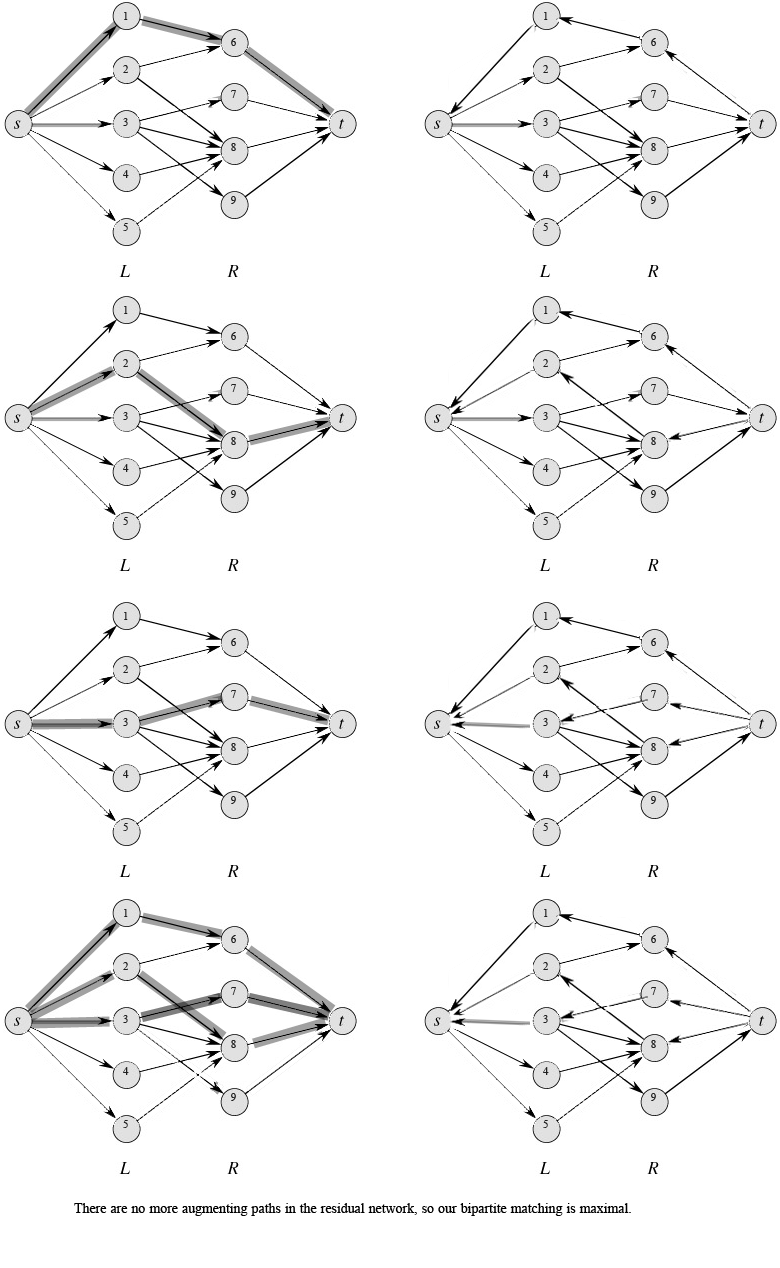
\includegraphics[scale=0.5]{fig268b.png}

\newpage

\subsection*{Problem 26-1}

{ \bf An $n \times n$ grid is an undirected graph consisting of $n$
rows and $n$ columns of vertices, as shown in Figure 26.11. We
denote the vertex in the $i^{th}$ row and the $j^{th}$ column by
$(i, j)$. All vertices in a grid have exactly four neighbors, except
for the boundary vertices, which are the points $(i, j)$ for which
$i = 1, i = n, j = 1, \text{ or } j = n$.

Given $m \leq n^2$ starting points $(x_1, y_1), (x_2, y_2),
...,(x_m, y_m)$ in the grid, the escape problem is to determine
whether or not there are $m$ vertex-disjoint paths from the starting
points to any $m$ different points on the boundary. For example, the
grid in Figure 26.11(a) has an escape, but the grid in Figure
26.11(b) does not.

\noindent a. Consider a flow network in which vertices, as well as
edges, have capacities. That is, the total positive flow entering
any given vertex is subject to a capacity constraint. Show that
determining the maximum flow in a network with edge and vertex
capacities can be reduced to an ordinary maximum-flow problem on a
flow network of comparable size. }

I like to think of this as a ``plumbing problem,'' where each edge
represents a pipe and each vertex represents a joint.

The vertex capacity limits the flow through a single vertex. So, the
total flow in and out of a single vertex cannot exceed the newly
introduced vertex capacity. If the vertex capacity {\em for all
vertices } is assigned so that the capacity exceeds the sum of the
incoming edge capacities, then the vertex capacities limit the
maximum flow algorithm in no way whatsoever.

This case is trivial, and because we are not in control of the
vertex capacities, I assume that a graph transformation is
appropriate. Because the vertices act like edges in so far as they
have flow constraints, why not transform all constraint vertices
into constraint edges, introducing two new traditional vertices to
bound each one? It works, but is it ``comparable size''?

$\text{Graph:} \rightarrow_5( 10 )\rightarrow_{15} \ \dashrightarrow\text{becomes}\dashrightarrow \ \text{Graph:} \rightarrow_5(\infty)\rightarrow_{10}(\infty)\rightarrow_{15}$\\

Each constraint vertex splits into two traditional (non-constraint)
vertices, which means that the size is bounded by a constant factor
of two. $O(2V) = O(V)$. Additionally, a new edge is introduced for
each vertex, which means that the graph grows by a factor up to $|V|
= O(V) \leq O(E)$ for any connected graph. So, the size of the
original graph with vertex constraints is $|V| + |E| = O(V+E)$, and
the size of the new graph is $3|V| + |E| = O(V+E)$. Asymptotic
equality is assumed to mean ``comparable size.''

\noindent { \bf b. Describe an efficient algorithm to solve the
escape problem. Analyze its running time.}

The \textbf{\em escape problem} can be modeled by a maximum flow
network in which the total number of matchings must equal the number
of starting points $m$. The super-source $s$ must be connected to
all $m$ starting points, and the super-sink $t$ must be connected to
all of the boundary points. Additionally, since the paths must be
vertex-disjoint (blocking), they must all have unit capacity.
(Taking a hint from (a), we split the unit vertex capacities into
new unit capacity edges with traditional vertex pairs.) Each
matching in the maximum flow network corresponds to an ``escape
route'' or vertex-disjoint path between the starting vertices and
the border vertices.

If the maximum flow algorithm results in $m$ matchings, then the
graph is said to be escapable. Otherwise, the graph is not escapable
for all $m$ starting vertices. This should be clear from the
definition of a vertex-disjoint path and the fact that all edge
capacities are initialized to {\large 1}.

From (a) we have that the graph is of upper bound $|V| \leq 2|v|$
(splitting) and $|E| \leq |e| + |v|$. Assume that the maximum flow
algorithm used is Edmunds-Karp. The running time of Edmunds-Karp as
given in the book is $O(V\ E^2)$. By a simple replacement, we see
that the running time is $O(2v\ (e+v)^2) = O(v\ (e^2+2ev+v^2)) =
O(e^2v+ev^2+v^3))$, a 3rd-degree polynomial of the original graph's
$e$ edges, and the original graph's $v$ vertices.

\newpage

\subsection*{Problem 26-3}

{\bf Professor Spock is consulting for NASA, which is planning a
series of space shuttle flights and must decide which commercial
experiments to perform and which instruments to have on board each
flight. For each flight, NASA considers a set $E = \{E_1, E_2, . . .
,E_m\}$ of experiments, and the commercial sponsor of experiment
$E_j$ has agreed to pay NASA $p_j$ dollars for the results of the
experiment. The experiments use a set $I = \{I_1, I_2, . . . ,I_n\}$
of instruments; each experiment $E_j$ requires all the instruments
in a subset $R_j \subseteq I$. The cost of carrying instrument $I_k$
is $c_k$ dollars. The professor's job is to find an efficient
algorithm to determine which experiments to perform and which
instruments to carry for a given flight in order to maximize the net
revenue, which is the total income from experiments performed minus
the total cost of all instruments carried.

Consider the following network $G$: The network contains a source
vertex $s$, instrument vertices $I_1, I_2, . . . ,I_n$, experiment
vertices $E_1, E_2, . . . ,E_m$, and a sink vertex $t$. For $k = 1,
2. . . ,n$, there is an edge $(s, I_k)$ of capacity $c_k$, and for
$j = 1, 2,. . . ,m$, there is an edge $(E_j, t)$ of capacity $p_j$.
For $k = 1, 2, . . . ,n$ and $j = 1, 2, . . . ,m$, if $I_k \epsilon
R_j$ , then there is an edge $(I_k, E_j)$ of infinite capacity.}

\noindent {\em Didn't we do this problem in class? I wish I had
written it down, now. I remember something similar.}

\noindent {\bf a. Show that if $E_j \epsilon T$ for a
finite-capacity cut $(S, T)$ of $G$, then $I_k \epsilon T$ for each
$I_k \epsilon R_j$. }

\noindent Assume $I_k \ni T$ for each $I_k \epsilon R_j$ Therefore,
$I_k \epsilon S$, because $(S,T)$ is a cut. We know $I_k \epsilon
R_j \rightarrow c(I_k, E_j) = \infty$ spans the cut. However, the
cut must be of {\em finite} capacity ($\Leftrightarrow$). Therefore,
our assumption is incorrect, and $I_k \epsilon T$.

\noindent {\bf b. Show how to determine the maximum net revenue from
the capacity of the minimum cut of $G$ and the given $p_j$ values. }

Intuitively, the answer is given by the sum $\sum_{j}\{p_j | E_j
\text{ experiment done}\} - \sum_{k}\{c_k | I_k \text{ instrument
used}\}$. We must find an equivalent way of expressing this in terms
of the capacity of the minimum cut, $c(S,T)$.

Calculate $\sum_jp_j$, the total profit for all possible
experiments. Subtract the total capacity of the cut. This should
yield the net revenue $R = \sum_jp_j - c(S,T)$. This works because
the capacity of the {\em minimum} cut represents the profits for
experiments {\em NOT} performed plus instrument expenses {\em that
ARE} incurred for an optimal solution. The difference is the optimal
net revenue.

\noindent {\bf c. Give an efficient algorithm to determine which
experiments to perform and which instruments to carry. Analyze the
running time of your algorithm in terms of $m, n,$ and $r =
\sum_{j=1}^m\mid R_j \mid$.}

\begin{enumerate}
  \item Use Edmunds-Karp to find a {\em minimum cut / maximum flow}.
  \item Calculate net revenue as given in (b).
  \item For all I and E values involved in the cut, add each instrument
and experiment to the list of involved items. The set of instruments
unused and experiments not performed is the Universe minus those
listed here.
\end{enumerate}

The book gives a running time of $O(V E^2)$ for Edmunds-Karp.
Because of the super-source and super-sink, $|V| = 1 + 1 + n + m =
O(n+m)$ and $|E| = n + m + r$. Doing a simple substitution, we have
$O((n+m)(n + m + r)^2)$, which expands as $O({m^3}+3 {m^2} n+3 m
{n^2}+{n^3}+2 {m^2} r+4 m n r+2 {n^2} r+m {r^2}+n {r^2})$. That is
the running time for part (1) only.

The net revenue can be calculated in $O(m + n)$ time, since $m$
experiments and $n$ instruments need to be checked and tallied, and
the profit vector $P$ is only $n$ units long. Similarly, the third
step is also $O(m + n)$. Overall efficiency is therefore $O({m^3}+
{m^2}n + m{n^2}+ {n^3} + {m^2}r + mnr + {n^2}r + m{r^2} + n{r^2})$,
where $r = \sum_{j=1}^m\mid R_j \mid$. Proving that this algorithm
is of optimal efficiency is left as an exercise to the reader
\smiley.

\newpage
\vspace*{4.5 in} \center{This class was fun! See you in
comprehensive exams.}

\end{document}
